\chapter{残余应力和变形}

残余应力和变形计算是多尺度问题,小尺度采用热循环计算,如图\ref{fig:4-1},大尺度采用固有应变法,如图\ref{fig:4-4}。在热循环计算中采用生死单元法,生死单元有两种情况,一种是计算区域是有真实的变化,需要添加网格单元,暂时称为激活单元,如图\ref{fig:4-2},另外一种情况是计算区域没有变化,通过改变材料系数增加单元,暂时称为静单元,我们采用激活单元和静单元的混合形式,逐层增加网格,然后再对每一层修改材料系数,如图\ref{fig:4-4}。计算区域如图\ref{fig:4-5},和图\ref{fig:4-6}中研究类似,具体几何参数可以调整。具体问题可以只计算热传导,或者计算热弹塑性,热弹塑性采用最简单的理想塑性本构。

\begin{figure}[!htbp]
  \centering
  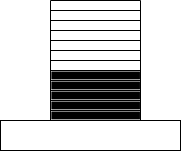
\includegraphics[height=3cm]{fig/4/1.png}
  \caption{热循环残余应力和变形计算}
  \label{fig:4-1}
\end{figure}

\begin{figure}[!htbp]
  \centering
  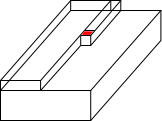
\includegraphics[height=3cm]{fig/4/2.png}
  \caption{激活单元}
  \label{fig:4-2}
\end{figure}

\begin{figure}[!htbp]
  \centering
  
\includegraphics[height=3cm]{fig/4/3.png}
  \caption{激活单元和静单元混合形式}
  \label{fig:4-3}
\end{figure}

\begin{figure}[!htbp]
  \centering
  
\includegraphics[height=3cm]{fig/4/4.png}
  \caption{固有应变法残余应力和变形计算}
  \label{fig:4-4}
\end{figure}

\begin{figure}[!htbp]
  \centering
  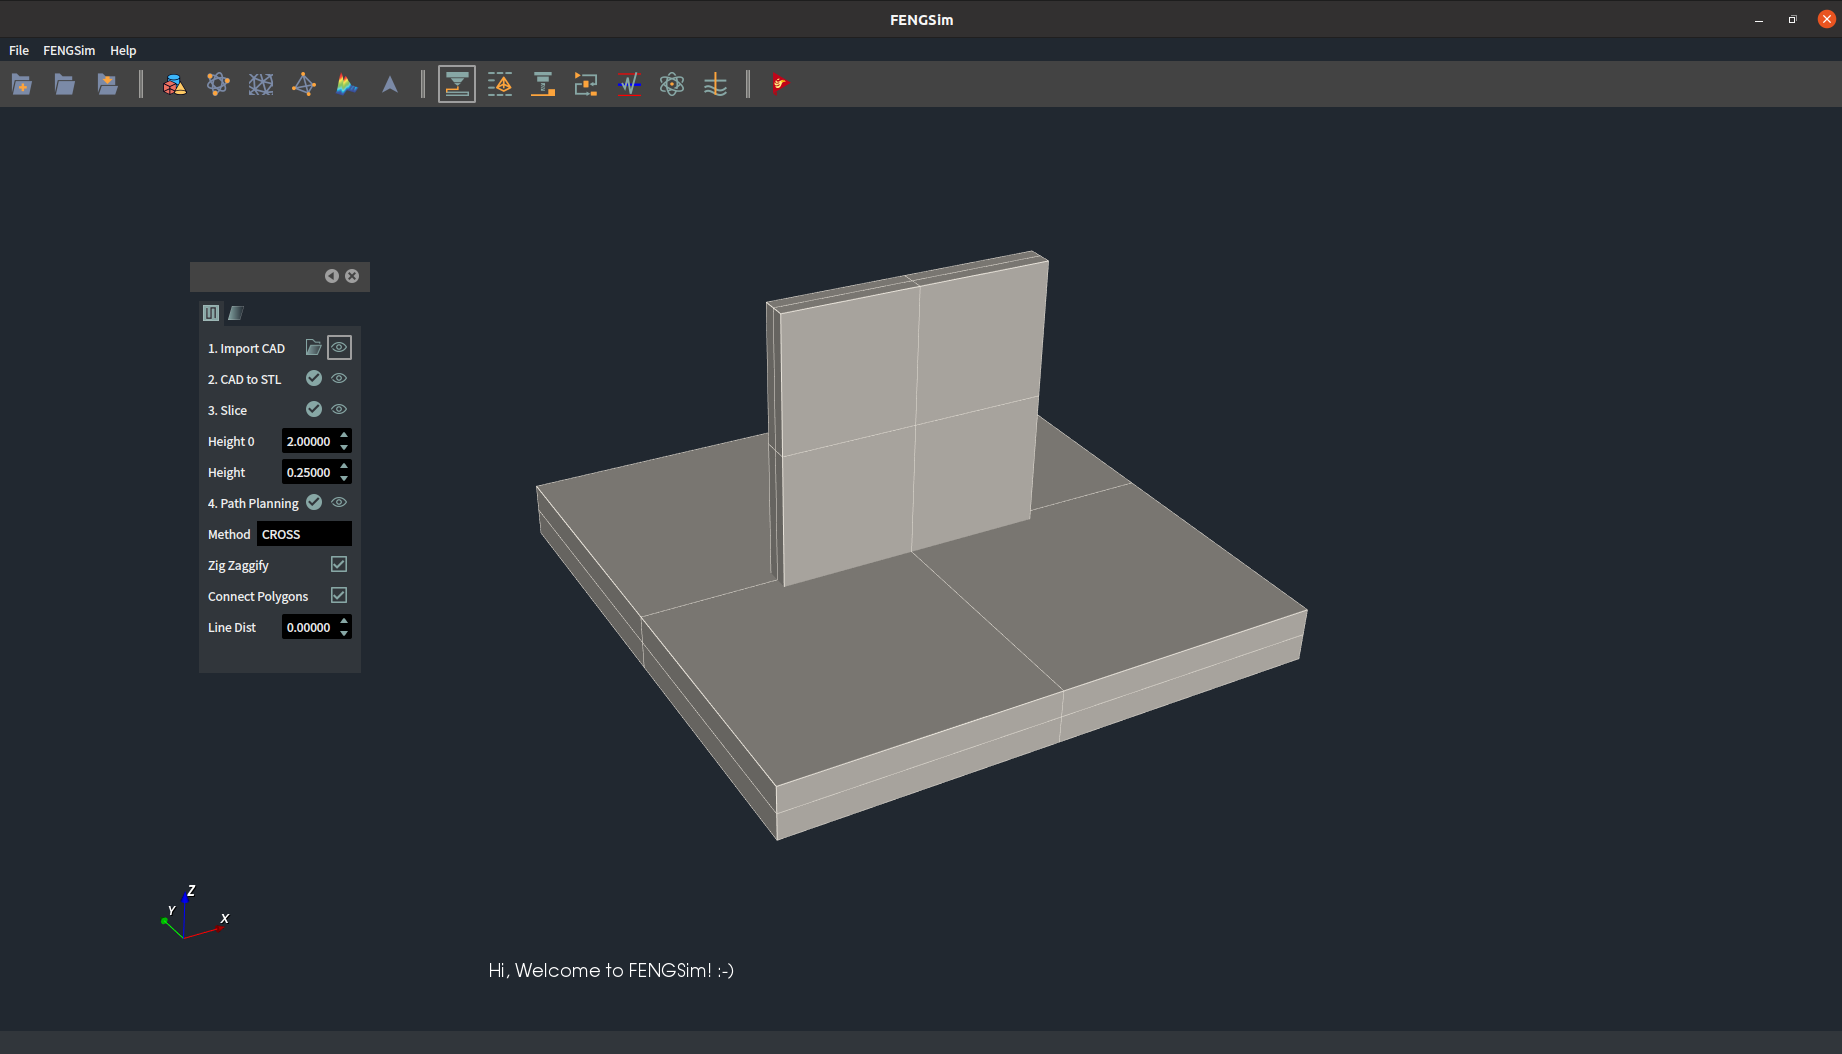
\includegraphics[height=5cm]{fig/4/5.png}
  \caption{CAD模型}
  \label{fig:4-5}
\end{figure}

\begin{figure}[!htbp]
  \centering
  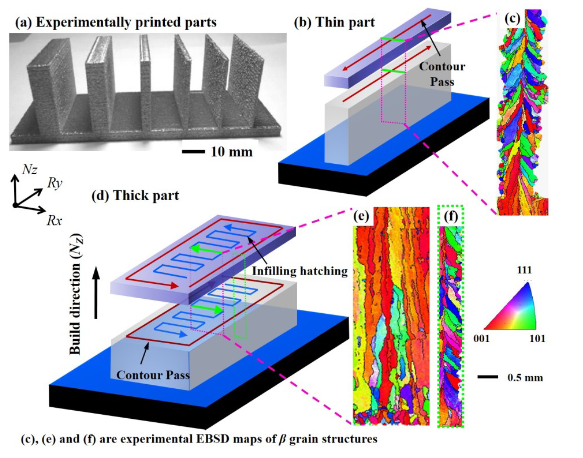
\includegraphics[height=5cm]{fig/4/6.png}
  \caption{固有应变法}
  \label{fig:4-6}
\end{figure}

\section{热弹塑性}

\section{小尺度热循环生死单元法}

\section{构件尺度固有应变法}
